\newpage
\section[Day 13: Riemann-Stieltjes Integral]{ Riemann-Stieltjes Integral }

\subsection{ Riemann-Stieltjes Integral }

    \begin{definition}{Riemann Integral}{16cm}
        For [a,b], let a = $x_0 \leq x_1 \leq ... \leq x_n$ = b
        and $\Delta x_i$ = $x_i - x_{i-1}$.

        Suppose real f is bounded.
        Then for each partition P, \{$x_0 , ... , x_n$\},

        let $m_i$ = inf f([$x_{i-1},x_i$]) and $M_i$ = sup f([$x_{i-1},x_i$]).
        
        Then let L(P,f) = $\sum_{i=1}^n$ $m_i \Delta x_i$
        and U(P,f) = $\sum_{i=1}^n$ $M_i \Delta x_i$. Thus, over all P:

        \hspace{0.5cm}
        Lower Riemann Integral:
        $\underline{\int}_a^b$ f(x) dx = sup L(P,f)

        \hspace{0.5cm}
        Upper Riemann Integral:
        $\overline{\int}_a^b$ f(x) dx = inf U(P,f)

        \vspace{0.2cm}

        If $\underline{\int}_a^b f(x) dx$
        = $\overline{\int}_a^b f(x) dx$ = $\int_a^b f(x) dx$, then
        f is {\color{lblue} Riemann-integrable}
        (i.e. f $\in$ $\mathscr{R}$).
        
        \vspace{0.2cm}

        Since f is bounded, there are m,M such that m $\leq$ f(x) $\leq$ M.

        Thus, m(b-a) $\leq$ L(P,f) $\leq$ U(P,f) $\leq$ M(b-a).
    \end{definition}



    \begin{figure}[h]
        \centering
        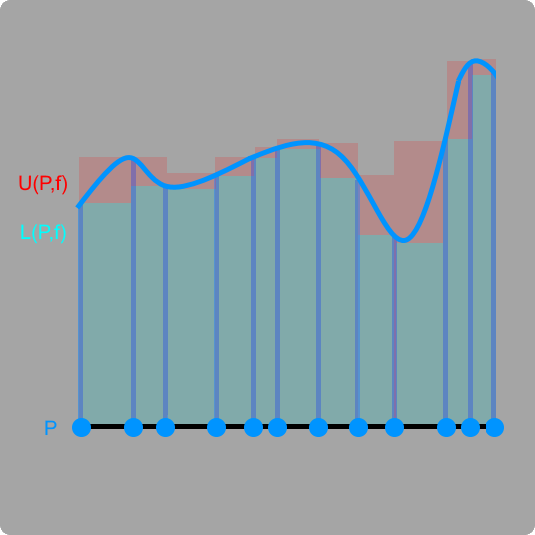
\includegraphics[scale=0.35]{Images/13.1.1.png}
    \end{figure}



    \begin{definition}{Riemann-Stieltjes Integral}{16cm}
        Let $\alpha$ be monotonically increasing on [a,b].
        
        Then for each partition P, let
        $\Delta \alpha_i$ = $\alpha(x_i)$ - $\alpha(x_{i-1})$.

        For real bounded f, let
        L(P,f,$\alpha$) = $\sum_{i=1}^n$ $m_i \Delta \alpha_i$
        and U(P,f,$\alpha$) = $\sum_{i=1}^n$ $M_i \Delta \alpha_i$.

        Thus, $\underline{\int}_a^b$ f(x) d$\alpha(x)$ = sup L(P,f,$\alpha$)
        and $\overline{\int}_a^b$ f(x) d$\alpha(x)$ = inf U(P,f,$\alpha$).

        \vspace{0.2cm}

        If $\underline{\int}_a^b$ f(x) d$\alpha(x)$
        = $\overline{\int}_a^b$ f(x) d$\alpha(x)$, then
        f $\in$ $\mathscr{R}(\alpha)$ with value $\int_a^b$ f(x) d$\alpha(x)$.        
    \end{definition}

    \vspace{0.5cm}

    

    \begin{definition}{Refinement}{16cm}
        Partition Q is a {\color{lblue} refinement} of P if P $\subset$ Q.

        For partitions $P_1, P_2$, then Q = $P_1 \cup P_2$ is the common refinement.
    \end{definition}

    \newpage



    \begin{wtheorem}{Refinements monotonically increase L(P,f)
    \& decrease U(P,f)}{16cm}
        If Q is a refinement of P, then:

        \hspace{0.5cm}
        L(P,f,$\alpha$) $\leq$ L(Q,f,$\alpha$)
        $\leq$ U(Q,f,$\alpha$) $\leq$ U(P,f,$\alpha$)
    \end{wtheorem}

    \begin{proof}
        Since Q is a refinement of P, then P $\subset$ Q.
        
        Suppose Q = P $\cup$ \{$x*$\} where
        P = \{$x_0,...,x_n$\} and Q = \{$x_0,...,x_{k-1},x*,x_k,..,x_n$\}.
        Regardless of anymore points, the process below will be analogous.

        \hspace{0.5cm}
        L(P,f,$\alpha$)
        = $\sum_{i=1}^{k-1}$ $m_i \Delta \alpha_i$
        + $m_{[x_{k-1},x_k]} [\alpha(x*) - \alpha(x_{k-1})]$
        
        \hspace{5.1cm}
        + $m_{[x_{k-1},x_k]} [\alpha(x_k) - \alpha(x*)]$
        + $\sum_{i=k+1}^n$ $m_i \Delta \alpha_i$

        \hspace{0.5cm}
        L(Q,f,$\alpha$)
        = $\sum_{i=1}^{k-1}$ $m_i \Delta \alpha_i$
        + $m_{[x_{k-1},x*]} [\alpha(x*) - \alpha(x_{k-1})]$

        \hspace{5.1cm}
        + $m_{[x*,x_k]} [\alpha(x_k) - \alpha(x_*)]$
        + $\sum_{i=k+1}^n$ $m_i \Delta \alpha_i$

        \hspace{0.5cm}
        Since $[x_{k-1},x*],[x*,x_k]$ $\subset$ $[x_{k-1},x_k]$, then
        $m_{[x_{k-1},x_k]} \leq m_{[x_{k-1},x*]}, m_{[x*,x_k]}$.
        Thus:

        \hspace{0.5cm}
        L(Q,f,$\alpha$) - L(P,f,$\alpha$)
        = ($m_{[x_{k-1,x*}]} - m_{[x_{k-1,x_k}]}$)$[\alpha(x*) - \alpha(x_{k-1})]$

        \hspace{4.5cm}
        + ($m_{[x_{k*,x_k}]} - m_{[x_{k-1,x_k}]}$)$[\alpha(x_k) - \alpha(x*)]$
        $\geq$ 0.

        \rule[0.1cm]{15cm}{0.01cm}

        \hspace{0.5cm}
        U(P,f,$\alpha$)
        = $\sum_{i=1}^{k-1}$ $M_i \Delta \alpha_i$
        + $M_{[x_{k-1},x_k]} [\alpha(x*) - \alpha(x_{k-1})]$
        
        \hspace{5.1cm}
        + $M_{[x_{k-1},x_k]} [\alpha(x_k) - \alpha(x*)]$
        + $\sum_{i=k+1}^n$ $M_i \Delta \alpha_i$

        \hspace{0.5cm}
        U(Q,f,$\alpha$)
        = $\sum_{i=1}^{k-1}$ $M_i \Delta \alpha_i$
        + $M_{[x_{k-1},x*]} [\alpha(x*) - \alpha(x_{k-1})]$

        \hspace{5.2cm}
        + $M_{[x*,x_k]} [\alpha(x_k) - \alpha(x_*)]$
        + $\sum_{i=k+1}^n$ $M_i \Delta \alpha_i$

        \hspace{0.5cm}
        Since $[x_{k-1},x*],[x*,x_k]$ $\subset$ $[x_{k-1},x_k]$, then
        $M_{[x_{k-1},x_k]} \geq M_{[x_{k-1},x*]}, M_{[x*,x_k]}$.
        Thus:

        \hspace{0.5cm}
        U(Q,f,$\alpha$) - U(P,f,$\alpha$)
        = ($M_{[x_{k-1,x*}]} - M_{[x_{k-1,x_k}]}$)$[\alpha(x*) - \alpha(x_{k-1})]$

        \hspace{4.5cm}
        + ($M_{[x_{k*,x_k}]} - M_{[x_{k-1,x_k}]}$)$[\alpha(x_k) - \alpha(x*)]$
        $\leq$ 0.
    \end{proof}



    \begin{figure}[h]
        \centering
        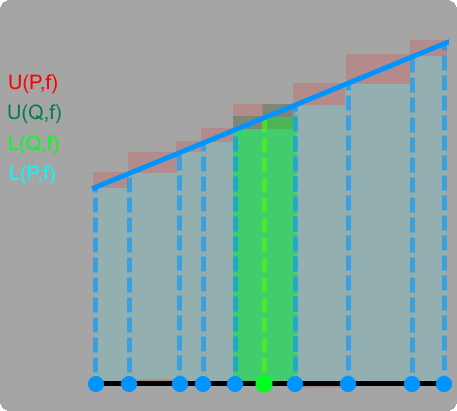
\includegraphics[scale=0.45]{Images/13.1.4.png}
    \end{figure}


    
    \begin{wtheorem}{Lower Riemann Integral $\leq$ Upper Riemann Integral}{16cm}
        $\underline{\int}_a^b f d \alpha$ $\leq$ $\overline{\int}_a^b f d \alpha$        
    \end{wtheorem}
    
    \begin{proof}
        For partitions $P_1,P_2$, let L($P_1,f,\alpha$) and U($P_2,f,\alpha$).
        Let P = $P_1 \cup P_2$. Thus:

        \hspace{0.5cm}
        L($P_1,f,\alpha$)
        $\leq$ L($P,f,\alpha$)
        $\leq$ U($P,f,\alpha$)
        $\leq$ U($P_2,f,\alpha$)

        Thus, over all partitions for $P_1$,
        $\underline{\int}_a^b f d \alpha$
        $\leq$ U($P_2,f,\alpha$)

        Thus, over all partitions for $P_2$,
        $\underline{\int}_a^b f d \alpha$
        $\leq$ $\overline{\int}_a^b f d \alpha$
    \end{proof}

    \newpage



    \begin{wtheorem}{Riemann-Integrability $\epsilon$ Definition}{16cm}
        f $\in$ $\mathscr{R}(\alpha)$ if and only if for every $\epsilon > 0$,
        there exists a partition P such that:

        \hspace{0.5cm}
        U($P,f,\alpha$) - L($P,f,\alpha$) $<$ $\epsilon$        
    \end{wtheorem}

    \begin{proof}
        If f $\in$ $\mathscr{R}(\alpha)$, then
        $\underline{\int}_a^ f d \alpha$
        = $\overline{\int}_a^b f d \alpha$
        = $\int_a^b f d \alpha$.
        For $\epsilon > 0$, there exists partitions $P_1,P_2$:

        \hspace{0.5cm}
        $\int_a^b$ $f d \alpha$ - L($P_1,f,\alpha$) $<$ $\frac{\epsilon}{2}$
        \hspace{1cm}
        U($P_2,f,\alpha$) - $\int_a^b$ $f d \alpha$ $<$ $\frac{\epsilon}{2}$

        Then for partition P = $P_1 \cup P_2$, then:

        \hspace{0.5cm}
        $\int_a^b$ $f d \alpha$ - L($P,f,\alpha$)
        $\leq$ $\int_a^b$ $f d \alpha$ - L($P_1,f,\alpha$)
        $<$ $\frac{\epsilon}{2}$

        \hspace{0.5cm}
        U($P,f,\alpha$) - $\int_a^b$ $f d \alpha$
        $\leq$ U($P_2,f,\alpha$) - $\int_a^b$ $f d \alpha$
        $<$ $\frac{\epsilon}{2}$

        Thus, U($P,f,\alpha$) - L($P,f,\alpha$) $<$ $\epsilon$.

        \rule[0.1cm]{15cm}{0.01cm}

        For $\epsilon > 0$, there is a partition P such that
        U($P,f,\alpha$) - L($P,f,\alpha$) $<$ $\epsilon$.

        Since L($P,f,\alpha$) $\leq$ $\underline{\int}_a^b f d \alpha$
        $\leq$ $\overline{\int}_a^b f d \alpha$ $\leq$ U($P,f,\alpha$), then
        $\overline{\int}_a^b f d \alpha$ - $\underline{\int}_a^b f d \alpha$
        $<$ $\epsilon$.
    \end{proof}

    \vspace{0.5cm}



    \begin{ltheorem}{Properties of Riemann-Integrability}{1.5cm}
        \item If f $\in$ $\mathscr{R}(\alpha)$, then
        U($Q,f,\alpha$) - L($Q,f,\alpha$) $<$ $\epsilon$ for 
        every refinement of P, Q

            \begin{proof}[15.5cm]
                By {\color{red} theorem 13.1.6}, for $\epsilon > 0$, there is a P
                such that:
                
                \hspace{0.5cm}
                U($P,f,\alpha$) - L($P,f,\alpha$) $<$ $\epsilon$.

                Then by {\color{red} theorem 13.1.4},
                for any refinement of P, Q, then:
                
                \hspace{0.5cm}
                U($Q,f,\alpha$) - L($Q,f,\alpha$) $<$ $\epsilon$.
            \end{proof}

        
        \item If f $\in$ $\mathscr{R}(\alpha)$ where
            P = \{$x_0,..,x_n$\} and $s_i,t_i$ $\in$ [$x_{i-1},x_i$],
            then:
        
            \hspace{1cm}
            $\sum_{i=1}^n$ $|f(s_i) - f(t_i)| \Delta \alpha_i$ $<$ $\epsilon$

            \begin{proof}[15.5cm]
                By {\color{red} theorem 13.1.6}, for $\epsilon > 0$,
                there is a P such that:

                \hspace{0.5cm}
                U($P,f,\alpha$) - L($P,f,\alpha$) $<$ $\epsilon$

                \hspace{0.5cm}
                $\sum_{i=1}^n$ $M_i \Delta \alpha_i$
                - $\sum_{i=1}^n$ $m_i \Delta \alpha_i$
                $<$ $\epsilon$

                Since $s_i,t_i$ $\in$ $[x_{i-1},x_i]$, then
                $m_i \leq f(s_i),f(t_i) \leq M_i$.

                Thus, $|f(s_i) - f(t_i)| \leq M_i - m_i$.

                \hspace{0.5cm}
                $\sum_{i=1}^n |f(s_i) - f(t_i)| \Delta \alpha_i$
                $\leq$ $\sum_{i=1}^n M_i - m_i \Delta \alpha_i$
                $\leq$ $\epsilon$    
            \end{proof}

        \item If f $\in$ $\mathscr{R}(\alpha)$ where
            P = \{$x_0,..,x_n$\} and $t_i$ $\in$ [$x_{i-1},x_i$],
            then:
        
            \hspace{1cm}
            $| \sum_{i=1}^n f(t_i) \Delta \alpha_i - \int_a^b f d \alpha |$
            $<$ $\epsilon$

            \begin{proof}[15.5cm]
                Since
                sup L($P,f,\alpha$) = $\underline{\int}_a^b f d \alpha$
                = $\int_a^b f d \alpha$
                = $\overline{\int}_a^b f d \alpha$ = inf U($P,f,\alpha$), then:

                \hspace{0.5cm}
                L($P,f,\alpha$) $\leq$ $\int_a^b f d \alpha$ $\leq$ U($P,f,\alpha$)

                Since $t_i$ $\in$ $[x_{i-1},x_i]$, then $m_i \leq f(t_i) \leq M_i$.
                Thus:
                
                \hspace{0.5cm}
                L($P,f,\alpha$) = $\sum_{i=1}^n$ $m_i \Delta \alpha_i$
                $\leq$ $\sum_{i=1}^n$ $f(t_i) \Delta \alpha_i$

                \hspace{5.2cm}
                $\leq$ $\sum_{i=1}^n$ $M_i \Delta \alpha_i$ = U($P,f,\alpha$)

                Thus, $| \sum_{i=1}^n$ $f(t_i) \Delta \alpha_i
                - \int_a^b f d \alpha |$
                $\leq$ U($P,f,\alpha$) - L($P,f,\alpha$)
                $<$ $\epsilon$.
            \end{proof}
    \end{ltheorem}

    \newpage





\subsection{ Riemann-Integrable Functions }

    \begin{wtheorem}{Continuous functions are Riemann-Integrable}{16cm}
        If f is continuous on [a,b], then f $\in$ $\mathscr{R}(\alpha)$
    \end{wtheorem}

    \begin{proof}
        For $\epsilon > 0$, choose $\eta > 0$ such that
        $[\alpha(b)-\alpha(a)] \eta < \epsilon$.
        Since f is continuous and [a,b] is compact, then f is uniformly continuous.
        Thus, for $\eta > 0$, there is a $\delta > 0$ such that
        for all x,t $\in$ [a,b] where $|x-t| < \delta$,
        then $|f(x) - f(t)| < \eta$.
        For partition P of [a,b] such that $\Delta x_i < \delta$ for all
        i=\{1,...,n\}, then $M_i - m_i \leq \eta$ for each i. Thus:
        
        \hspace{0.5cm}
        U($P,f,\alpha$) - L($P,f,\alpha$)
        = $\sum_{i=1}^n (M_i - m_i) \Delta \alpha_i$
        $\leq$ $\sum_{i=1}^n \eta \Delta \alpha_i$
        = $\eta [\alpha(b) - \alpha(a)]$
        $<$ $\epsilon$
    \end{proof}

    \vspace{0.5cm}



    \begin{wtheorem}{Monotonic functions are Riemann-Integrable}{16cm}
        If f is monotonic on [a,b] and $\alpha$ is continuous on [a,b], then
        f $\in$ $\mathscr{R}(\alpha)$        
    \end{wtheorem}
    
    \begin{proof}
        Since $\alpha$ is continuous on [a,b],
        let $\Delta \alpha_i$ = $\frac{\alpha(b) - \alpha(a)}{n}$
        where n $\in$ $\mathbb{Z}_+$

        Let partition P = \{$\alpha(x_0),...,\alpha(x_n)$\}.
        Suppose f is monotonically increasing. Thus:
        
        \hspace{0.5cm}
        U($P,f,\alpha$) - L($P,f,\alpha$)
        = $\sum_{i=1}^n (M_i - m_i) \Delta \alpha_i$
        = $\frac{\alpha(b) - \alpha(a)}{n} \sum_{i=1}^n (M_i - m_i)$

        \hspace{4.5cm}
        = $\frac{\alpha(b) - \alpha(a)}{n} \sum_{i=1}^n [f(x_i) - f(x_{i-1})]$
        = $\frac{\alpha(b) - \alpha(a)}{n} [f(b)-f(a)]$
        
        For $\epsilon > 0$, there exists a n such that
        $\frac{\alpha(b) - \alpha(a)}{n} [f(b)-f(a)] < \epsilon$
        so f $\in$ $\mathscr{R}(\alpha)$.
        
        If f is monotonically decreasing, then
        $\sum_{i=1}^n (M_i - m_i)$ = $\sum_{i=1}^n [f(x_{i-1}) - f(x_i)]$.
    \end{proof}

    \vspace{0.5cm}



    \begin{wtheorem}{Bounded functions with finite discontinuities
    are Riemann-Integrable}{16cm}
        If f is bounded on [a,b] with finitely many discontinuities
        and $\alpha$ is continuous at every discontinuity, then
        f $\in$ $\mathscr{R}(\alpha)$        
    \end{wtheorem}

    \begin{proof}
        Since f is bounded, let M = sup $|f(x)|$ and
        E be the set of discontinuities of f.

        Since E is finite and $\alpha$ is continuous over E, then
        for $\epsilon > 0$, there are finitely many disjoint
        $[u_j,v_j]$ where $\sum [\alpha(v_j) - \alpha(u_j)] < \epsilon$ which cover E.

        Let K = [a,b] $\backslash$ $\cup$ $(u_j,v_j)$ which is compact.
        Since f is continuous over compact K, then f is uniformly continuous
        over K.
        Thus, for $\epsilon > 0$, there is a $\delta > 0$ such that for
        s,t $\in$ K where $|s-t| < \delta$, then $|f(s) - f(t)| < \epsilon$.

        Let partition P = \{$x_0,...,x_n$\} of [a,b] where
        each $\Delta x_i$ $<$ $\delta$ and if x $\in$ 
        $(u_j,v_j)$ $\not \in$ P, but $u_j,v_j$ $\in$ P.
        Thus, $M_i - m_i \leq 2M$ for each i and
        $M_i - m_i \leq \epsilon$ unless
        $x_{i-1}$ is a $u_j$, then:

        \hspace{0.1cm}
        U($P,f,\alpha$) - L($P,f,\alpha$)
        = $\sum_{i=1}^n (M_i - m_i) \Delta \alpha_i$
        = $\sum_{K} (M_i - m_i) \Delta \alpha_i$
            + $\sum_{K^c} (M_i - m_i) \Delta \alpha_i$

        \hspace{3.9cm}
        $\leq$ $\epsilon \sum_{K} \Delta \alpha_i$
            + $2M \sum_{K^c} \Delta \alpha_i$
        $\leq$ $[\alpha(b) - \alpha(a)]\epsilon + 2M\epsilon$
    \end{proof}



    \begin{figure}[h]
        \centering
        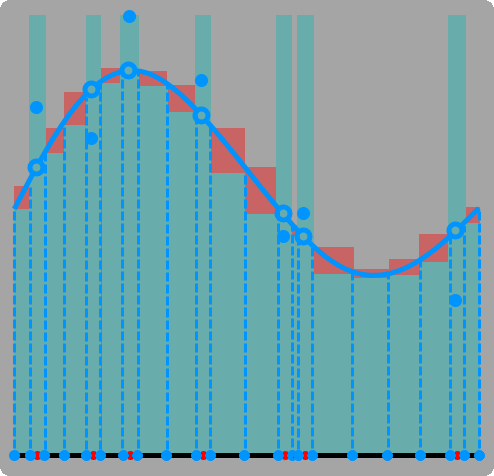
\includegraphics[scale=0.35]{Images/13.2.3.png}
    \end{figure}

    \newpage



    \begin{wtheorem}
    {Composite of continuous-integrable functions are Riemann-Integrable}{16cm}
        If f $\in$ $\mathscr{R}(\alpha)$ on [a,b] where f $\in$ [m,M] and
        $\phi$ is continuous on [m,M] such that h(x) = $\phi$(f(x)), then
        h $\in$ $\mathscr{R}(\alpha)$        
    \end{wtheorem}

    \begin{proof}
        Since $\phi$ is continuous and [m,M] is compact, then $\phi$
        is uniformly continuous.
        Thus, for $\epsilon > 0$, there is a $0 < \delta < \epsilon$ such that
        for all s,t $\in$ [m,M] where $|s-t| \leq \delta$, then
        $|\phi(s) - \phi(t)| < \epsilon$.
        
        Since f $\in$ $\mathscr{R}(\alpha)$, there is a partition P
        = \{$x_0,...,x_n$\} such that:
        
        \hspace{0.5cm}
        U($P,f,\alpha$) - L($P,f,\alpha$) $<$ $\delta^2$

        For each i=\{1,...,n\}, let i $\in$ A if $M_i - m_i < \delta$
        and i $\in$ B if $M_i - m_i \geq \delta$.

        Let $m_i^*$ = inf $\phi(f([x_{i-1},x_i]))$
        and $M_i^*$ = sup $\phi(f([x_{i-1},x_i]))$.

        For A, since $M_i - m_i < \delta$, then
        $M_i^* - m_i^* \leq \epsilon$.

        For B, $M_i^* - m_i^* \leq 2K$ where K = sup$_{[m,M]}$ $|\phi|$.

        \hspace{0.5cm}
        $\delta \sum_{i \in B} \Delta \alpha_i$
        $\leq$ $\sum_{i \in B} (M_i - m_i) \Delta \alpha_i$
        $<$ $\delta^2$

        \hspace{0.5cm}
        $\sum_{i \in B} \Delta \alpha_i$ $\leq$ $\delta$ $<$ $\epsilon$

        Thus:

        \hspace{0.5cm}
        U($P,h,\alpha$) - L($P,h,\alpha$)
        = $\sum_{i \in A} (M_i^* - m_i^*) \Delta \alpha_i$
            + $\sum_{i \in B} (M_i^* - m_i^*) \Delta \alpha_i$

        \hspace{4.5cm}
        $\leq$ $\epsilon \sum_{i \in A} \Delta \alpha_i$
                + $2K \sum_{i \in B} \Delta \alpha_i$
        
        \hspace{4.5cm}
        $\leq$ $\epsilon[\alpha(b) - \alpha(a)]$
                + $2K \epsilon$
        $<$ $\epsilon[\alpha(b) - \alpha(a) + 2K]$
    \end{proof}

    \vspace{0.5cm}





\subsection{ Integral Properties }

    \begin{ltheorem}{Integral Additive Properties}{1.5cm}
        \item If $f_1,f_2$ $\in$ $\mathscr{R}(\alpha)$ on [a,b] and constant c,
        then $f_1 + f_2,cf_1$ $\in$ $\mathscr{R}(\alpha)$ and

            \hspace{0.5cm}
            $\int_a^b$ $f_1 + f_2$ $d\alpha$
            = $\int_a^b$ $f_1$ $d\alpha$ + $\int_a^b$ $f_2$ $d\alpha$

            \hspace{0.5cm}
            $\int_a^b$ $cf_1$ $d\alpha$ = $c \int_a^b$ $f_1$ $d\alpha$

            \begin{proof}[15.5cm]
                Since $f_1,f_2$ $\in$ $\mathscr{R}(\alpha)$, then there are
                partitions $P_1,P_2$ such that for $\epsilon > 0$:

                \hspace{0.5cm}
                U($P_1,f_1,\alpha$) - L($P_1,f_1,\alpha$) $<$ $\frac{\epsilon}{2}$
                \hspace{1cm}
                U($P_2,f_2,\alpha$) - L($P_2,f_2,\alpha$) $<$ $\frac{\epsilon}{2}$

                Thus for partition P = $P_1 \cup P_2$:

                \hspace{0.5cm}
                U($P,f_1,\alpha$) + U($P,f_2,\alpha$)
                - L($P,f_1,\alpha$) - L($P,f_2,\alpha$)
                $<$ $\epsilon$

                \hspace{0.5cm}
                U($P,f_1+f_2,\alpha$) - L($P,f_1+f_2,\alpha$) $<$ $\epsilon$

                For any partition Q:

                \hspace{0.5cm}
                L($Q,f_1,\alpha$) + L($Q,f_2,\alpha$)
                $\leq$ L($Q,f_1+f_2,\alpha$)
                $\leq$ U($Q,f_1+f_2,\alpha$)

                \hspace{5cm}
                $\leq$ U($Q,f_1,\alpha$) + U($Q,f_2,\alpha$)

                Thus, $f_1+f_2$ $\in$ $\mathscr{R}(\alpha)$ where:

                \hspace{0.5cm}
                $\int_a^b$ $f_1$ $d\alpha$
                + $\int_a^b$ $f_2$ $d\alpha$
                = $\underline{\int}_a^b$ $f_1$ $d\alpha$
                + $\underline{\int}_a^b$ $f_2$ $d\alpha$
                $\leq$ $\underline{\int}_a^b$ $f_1+f_2$ $d\alpha$

                \hspace{4.3cm}
                = $\int_a^b$ $f_1+f_2$ $d\alpha$
                = $\overline{\int}_a^b$ $f_1+f_2$ $d\alpha$
                
                \hspace{4.3cm}
                $\leq$ $\overline{\int}_a^b$ $f_1$ $d\alpha$
                + $\overline{\int}_a^b$ $f_2$ $d\alpha$
                = $\int_a^b$ $f_1$ $d\alpha$
                + $\int_a^b$ $f_2$ $d\alpha$

                Proof for $cf_1$ is analogous by replacing $\frac{\epsilon}{2}$
                with $\frac{\epsilon}{c}$.                
            \end{proof}

    \item If $f_1,f_2$ $\in$ $\mathscr{R}(\alpha)$ and $f_1(x) \leq f_2(x)$
    on [a,b], then $\int_a^b$ $f_1$ $d\alpha$ $\leq$ $\int_a^b$ $f_2$ $d\alpha$

        \begin{proof}[15.5cm]
            Since $f_1,f_2$ $\in$ $\mathscr{R}(\alpha)$, then by part a,
            0 $\leq$ $\int_a^b f_2-f_2 d\alpha$
            = $\int_a^b f_2 d\alpha$ - $\int_a^b f_1 d\alpha$.
        \end{proof}

        \newpage

    \item If $f$ $\in$ $\mathscr{R}(\alpha)$ on [a,b] and c $\in$ (a,b),
    then f $\in$ $\mathscr{R}(\alpha)$ on [a,c],[c,b] and
        
        \hspace{0.5cm}
        $\int_a^c$ $f$ $d\alpha$ + $\int_c^b$ $f$ $d\alpha$
        = $\int_a^b$ $f$ $d\alpha$

        \begin{proof}[15.5cm]
            Since $f \in \mathscr{R}(\alpha)$ on [a,b], there is a
            partition P of [a,b] such that for $\epsilon > 0$:

            \hspace{0.5cm}
            U($P,f,\alpha$) - L($P,f,\alpha$) $<$ $\epsilon$

            For partition P of [a,b], let refinement of P, Q = P $\cup$ \{c\}.
            Thus:

            \hspace{0.5cm}
            L($P,f,\alpha$)
            $\leq$ L($Q,f,\alpha$)
            $\leq$ U($Q,f,\alpha$)
            $\leq$ U($P,f,\alpha$)

            Thus, let A = (P $<$ c) $\cup$ c $\in$ [a,c]
            and B = c $\cup$ (c $<$ P) $\in$ (c,b):  

            \hspace{0.5cm}
            L($Q,f,\alpha$)
            = $\sum_Q$ $m_q \Delta \alpha_q$

            \hspace{2.4cm}
            $\leq$ $\sum_A$ $m_a \Delta \alpha_a$ + $\sum_B$ $m_b \Delta \alpha_b$
            = L($A,f,\alpha$) + L($B,f,\alpha$)

            \hspace{0.5cm}
            U($Q,f,\alpha$)
            = $\sum_Q$ $M_q \Delta \alpha_q$

            \hspace{2.4cm}
            $\geq$ $\sum_A$ $M_a \Delta \alpha_a$ + $\sum_B$ $M_b \Delta \alpha_b$
            = U($A,f,\alpha$) + U($B,f,\alpha$)

            Since Q is a refinement of P, then
            U($Q,f,\alpha$) - L($Q,f,\alpha$) $<$ $\epsilon$. Thus:

            \hspace{0.5cm}
            0 $\leq$ U($A,f,\alpha$) + U($B,f,\alpha$)
            - L($A,f,\alpha$) - L($B,f,\alpha$) $<$ $\epsilon$

            \hspace{0.5cm}
            U($A,f,\alpha$) - L($A,f,\alpha$) $<$ $\epsilon$
            \hspace{1cm}
            U($B,f,\alpha$) - L($B,f,\alpha$) $<$ $\epsilon$

            Thus, $f \in \mathscr{R}(\alpha)$ on [a,c],[c,b] where:

            \hspace{0.5cm}
            $\underline{\int}_a^b$ $f$ $d\alpha$
            $\leq$ $\underline{\int}_a^c$ $f$ $d\alpha$
            + $\underline{\int}_c^b$ $f$ $d\alpha$
            = $\int_a^c$ $f$ $d\alpha$ + $\int_c^b$ $f$ $d\alpha$
            
            \hspace{2.1cm}
            = $\overline{\int}_a^c$ $f$ $d\alpha$
            + $\overline{\int}_c^b$ $f$ $d\alpha$
            $\leq$ $\overline{\int}_a^b$ $f$ $d\alpha$

            Since $\underline{\int}_a^b$ $f$ $d\alpha$,
            $\overline{\int}_a^b$ $f$ $d\alpha$
            = $\int_a^b$ $f$ $d\alpha$, then
            $\int_a^b$ $f$ $d\alpha$
            = $\int_a^c$ $f$ $d\alpha$ + $\int_c^b$ $f$ $d\alpha$.
        \end{proof}

    \item If $f$ $\in$ $\mathscr{R}(\alpha_1)$,$\mathscr{R}(\alpha_2)$ and
    constant c, then $f$ $\in$ $\mathscr{R}(\alpha_1+\alpha_2)$,
    $f$ $\in$ $\mathscr{R}(c\alpha_1)$ and

        \hspace{0.5cm}
        $\int_a^b$ $f$ $d(\alpha_1 + \alpha_2)$
        = $\int_a^b$ $f$ $d\alpha_1$ + $\int_a^b$ $f$ $d\alpha_2$

        \hspace{0.5cm}
        $\int_a^b$ $f$ $d(c\alpha_1)$
        = $c \int_a^b$ $f$ $d\alpha_1$

        \begin{proof}[15.5cm]
            Since $f \in \mathscr{R}(\alpha_1),\mathscr{R}(\alpha_2)$,
            then there are partitions $P_1,P_2$ where for $\epsilon > 0$:

            \hspace{0.5cm}
            U($P_1,f,\alpha_1$) - L($P_1,f,\alpha_1$) $<$ $\frac{\epsilon}{2}$
            \hspace{1cm}
            U($P_2,f,\alpha_2$) - L($P_2,f,\alpha_2$) $<$ $\frac{\epsilon}{2}$

            Thus, for partition P = $P_1 \cup P_2$:

            \hspace{0.5cm}
            $\sum_{i=1}^n$ $(M_i - m_i) \Delta \alpha_{1i}$
            $<$ $\frac{\epsilon}{2}$
            \hspace{1.5cm}
            $\sum_{i=1}^n$ $(M_i - m_i) \Delta \alpha_{2i}$
            $<$ $\frac{\epsilon}{2}$

            \hspace{2cm}
            $\sum_{i=1}^n$ $(M_i - m_i)
                            (\Delta \alpha_{1i} + \Delta \alpha_{2i})$
            $<$ $\epsilon$

            \hspace{2cm}
            U($P,f,\alpha_1+\alpha_2$) - L($P,f,\alpha_1+\alpha_2$)
            $<$ $\epsilon$

            For any partition Q:

            \hspace{0.5cm}
            L($Q,f,\alpha_1$) + L($Q,f,\alpha_2$)
            $\leq$ L($Q,f,\alpha_1+\alpha_2$)
            
            \hspace{5.1cm}
            $\leq$ U($Q,f,\alpha_1+\alpha_2$)

            \hspace{5.1cm}
            $\leq$ U($Q,f,\alpha_1$) + U($Q,f,\alpha_2$)

            Thus, $f \in \mathscr{R}(\alpha_1+\alpha_2)$ where:

            \hspace{0.5cm}
            $\int_a^b$ $f$ $d\alpha_1$ + $\int_a^b$ $f$ $d\alpha_2$
            = $\underline{\int}_a^b$ $f$ $d\alpha_1$
            + $\underline{\int}_a^b$ $f$ $d\alpha_2$
            $\leq$ $\underline{\int}_a^b$ $f$ $d(\alpha_1+\alpha_2)$

            \hspace{4.4cm}
            = $\int_a^b$ $f$ $d(\alpha_1+\alpha_2)$
            = $\overline{\int}_a^b$ $f$ $d(\alpha_1+\alpha_2)$

            \hspace{4.4cm}
            $\leq$ $\overline{\int}_a^b$ $f$ $d\alpha_1$
            + $\overline{\int}_a^b$ $f$ $d\alpha_2$
            = $\int_a^b$ $f$ $d\alpha_1$ + $\int_a^b$ $f$ $d\alpha_2$

            Proof for $c\alpha_1$ is analogous by replacing
            $\frac{\epsilon}{2}$ with $\frac{\epsilon}{c}$.
        \end{proof}
    \end{ltheorem}
    
    \newpage



    \begin{ltheorem}{Integral Multiplicative Properties}{1.5cm}
        \item If f,g $\in$ $\mathscr{R}(\alpha)$ on [a,b], then
        fg $\in$ $\mathscr{R}(\alpha)$
    
            \begin{proof}[15.5cm]
                Since f,g $\in$ $\mathscr{R}(\alpha)$, then
                f+g,f-g $\in$ $\mathscr{R}(\alpha)$.
                By {\color{red} theorem 13.2.4}, let
                $\phi(t)$ = $t^2$ which is continuous so
                $\phi(f+g)$ = $(f+g)^2$,$\phi(f-g)$ = $(f-g)^2$ $\in$
                $\mathscr{R}(\alpha)$.

                Thus, 4fg = $(f+g)^2 - (f-g)^2$ $\in$ $\mathscr{R}(\alpha)$.                
            \end{proof}

        \item If f $\in$ $\mathscr{R}(\alpha)$ on [a,b], then
        $|f|$ $\in$ $\mathscr{R}(\alpha)$ where
        $|\int_a^b f d\alpha|$ $\leq$ $\int_a^b |f| d\alpha$

            \begin{proof}[15.5cm]
                By {\color{red} theorem 13.2.4}, let
                $\phi(t)$ = $|t|$ which is continuous so $|f|$ $\in$
                $\mathscr{R}(\alpha)$.

                Then choose c = $\pm 1$ such that $c \int f d\alpha$ $\geq$ 0. Then:

                \hspace{0.5cm}
                $|\int f d\alpha|$
                = $c \int f d\alpha$
                = $\int cf d\alpha$
                $\leq$ $\int |f| d\alpha$
            \end{proof}    
    \end{ltheorem}

    \vspace{0.5cm}





\subsection{ Change of Variable }

    \begin{definition}{Unit Step Function}{16cm}
        I(x) =
        $
        \begin{cases}
            0 & x \leq 0 \\
            1 & x > 0
        \end{cases}
        $
    \end{definition}

    \vspace{0.5cm}



    \begin{wtheorem}{Integrating f over I centered at s}{16cm}
        If f is bounded on [a,b] and continuous at s $\in$ (a,b) where
        $\alpha(x)$ = I(x-s), then:

        \hspace{0.5cm}
        $\int_a^b$ $f$ $d\alpha$ = f(s)
    \end{wtheorem}

    \begin{intuition}
        If x $<$ s $<$ y, then $\Delta I$ = I($y-s$) - I($x-s$) = 1 - 0 = 1
        else $\Delta I$ = 0.

        So, $f(x) d\alpha(x)$ $\approx$ $f(x) \Delta I$
        have only $f(s) \Delta I$ = $f(s)$ since the others $\Delta I$ = 0.
    \end{intuition}

    \vspace{0.1cm}
    
    \begin{proof}
        For partition P = \{$x_0,x_1,x_2,x_3$\} where $x_1$ = s:

        \hspace{0.5cm}
        L($P,f,\alpha$) = $m_2$
        \hspace{1cm}
        U($P,f,\alpha$) = $M_2$

        Since f is continuous at s, then for $\epsilon > 0$, there is a $\delta > 0$
        where for all x $\in$ [s,s+$\delta$],
        
        then $|f(x)-f(s)| < \frac{\epsilon}{2}$.
        Thus, $M_2 - m_2$ $<$ $\frac{\epsilon}{2} + \frac{\epsilon}{2}$
        = $\epsilon$ so $\int f d\alpha$ exist where:

        \hspace{0.5cm}
        $f(s) - m_2$ $<$ $\frac{\epsilon}{2}$
        so $\underline{\int} f d\alpha$ = f(s)
        \hspace{1cm}
        $M_2 - f(s)$ $<$ $\frac{\epsilon}{2}$
        so $\overline{\int} f d\alpha$ = f(s)
    \end{proof}

    

    \begin{figure}[h]
        \centering
        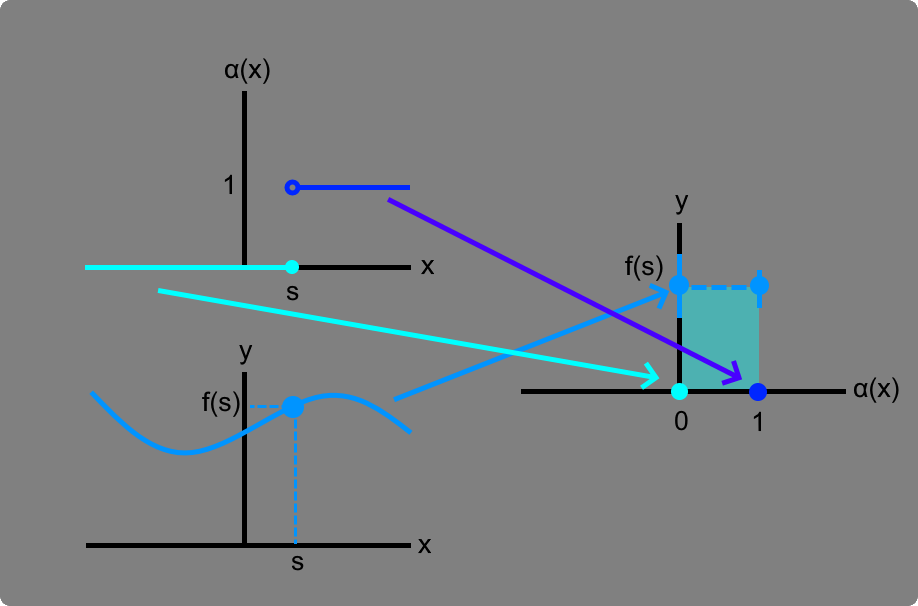
\includegraphics[scale=0.3]{Images/13.4.2.png}
    \end{figure}

    \newpage



    \begin{wtheorem}{Integrating f over a Step function}{16cm}
        If $\sum c_n$ converges where $c_n \geq 0$,
        distinct points \{$s_n$\} $\in$ (a,b), and
        $\alpha(x)$ = $\sum c_n I(x-s_n)$. Then for continuous f on [a,b]:

        \hspace{0.5cm}
        $\int_a^b f d\alpha$ = $\sum c_n f(s_n)$
    \end{wtheorem}

    \begin{intuition}
        Similar to {\color{red} theorem 13.4.2}, but over a step function.
        The \{$s_n$\} determines where the steps are and the \{$\sum c_n$\}
        determines the value at each step.

        Thus, $f(x) d\alpha(x)$ have only:

        \hspace{0.5cm}
        $f(s_n) \cdot (\text{value}_{\text{current step}}
                        - \text{value}_{\text{previous step}})$
        = $f(s_n) \cdot (\sum c_n - \sum c_{n-1})$
        = $f(s_n) \cdot c_n$
    \end{intuition}

    \vspace{0.1cm}
    
    \begin{proof}
        Since $\alpha(x)$ = $\sum c_n I(x-s_n)$ $\leq$ $\sum c_n$, then
        by the comparison test, $\alpha(x)$ converges.

        Since $c_n,I(x-s_n) \geq 0$, then $\alpha(x)$ is monotonic.

        Since a $<$ $s_n$ for any n, then
        $\alpha(a)$ = $\sum c_n I(a-s_n)$ = $\sum c_n 0$ = 0.

        Since b $>$ $s_n$ for any n, then
        $\alpha(a)$ = $\sum c_n I(b-s_n)$ = $\sum c_n 1$ = $\sum c_n$.

        Since $\sum c_n$ converges, then for $\epsilon > 0$, there is a N
        such that $\sum_{n=N+1}^{\infty} c_n < \epsilon$.

        Let $\alpha_1(x)$ = $\sum_{n=1}^N c_n I(x-s_n)$
        and $\alpha_2(x)$ = $\sum_{n=N+1}^{\infty} c_n I(x-s_n)$.
        By {\color{red} theorem 13.4.2}:
        
        \hspace{0.5cm}
        $\int_a^b f d\alpha_1$
        = $\int_a^b f d(\sum_{n=1}^N c_n I(x-s_n))$
        = $\sum_{n=1}^N$ $c_n f(s_n)$

        \hspace{0.5cm}
        $|\int_a^b f d\alpha_2|$
        = $\sum_{n=N+1}^{\infty}$ $c_n f(s_n)$
        $\leq$ $\sum_{n=N+1}^{\infty}$ $c_n$sup($|f(x)|$)
        = sup($|f(x)|$)$\epsilon$

        Thus, $\int f d\alpha$
        = $\int f d(\alpha_1+\alpha_2)$
        = $\int f d\alpha_1$ + $\int f d\alpha_2$
        = $\sum_{n=1}^N$ $c_n f(s_n)$ + sup($|f(x)|$)$\epsilon$    
    \end{proof}

    \vspace{0.5cm}



    \begin{wtheorem}{$\int_a^b$ $f$ d$\alpha$
    = $\int_a^b$ $f(x) \alpha'(x)$ dx}{16cm}
        If $\alpha'$ $\in$ $\mathscr{R}$ on [a,b] and
        f is real, bounded on [a,b], then f $\in$ $\mathscr{R}(\alpha)$
        if and only if f$\alpha'$ $\in$ $\mathscr{R}$. Then:

        \hspace{0.5cm}
        $\int_a^b$ $f$ d$\alpha$ = $\int_a^b$ $f(x) \alpha'(x)$ dx        
    \end{wtheorem}

    \begin{intuition}
        If $\alpha$ is differentiable on [x,y], then by the Mean Value Theorem,
        there is a t $\in$ [x,y]:

        \hspace{0.5cm}
        $\alpha(x) - \alpha(y)$ = $\alpha'(t) \cdot (x-y)$

        Since
        $d\alpha$
        $\approx$ $\Delta \alpha(x)$
        = $\alpha'(t) \Delta x$
        $\approx$ $\alpha'(x)$ dx,
        then $\int_a^b$ $f$ d$\alpha$ = $\int_a^b$ $f(x) \alpha'(x)$ dx.
    \end{intuition}

    \vspace{0.1cm}

    \begin{proof}
        Since $\alpha' \in \mathscr{R}$, then $\epsilon > 0$, there is a
        partition P = \{$x_0,...,x_n$\} such that:
        
        \hspace{0.5cm}
        U($P,\alpha'$) - L($P,\alpha'$) $<$ $\epsilon$

        By the Mean Value Theorem, there are $t_i$ $\in$ [$x_{i-1},x_i$]
        such that $\Delta \alpha_i$ = $\alpha'(t_i) \Delta x_i$.

        Then for $s_i$ $\in$ [$x_{i-1},x_i$]:

        \hspace{0.5cm}
        $\sum_{i=1}^n$ $|\alpha'(s_i) - \alpha'(t_i)| \Delta x_i$
        $\leq$ U($P,\alpha'$) - L($P,\alpha'$) $<$ $\epsilon$

        Let M = sup($|f(x)|$). Since
        $\sum_{i=1}^n$ $f(s_i) \Delta \alpha_i$
        = $\sum_{i=1}^n$ $f(s_i) \alpha'(t_i) \Delta x_i$, then:

        \hspace{0.5cm}
        $|\sum_{i=1}^n$ $f(s_i) \Delta \alpha_i
            - \sum_{i=1}^n$ $f(s_i) \alpha'(s_i) \Delta x_i|$

        \hspace{0.5cm}
        = $|\sum_{i=1}^n$ $f(s_i) \alpha'(t_i) \Delta x_i
            - \sum_{i=1}^n$ $f(s_i) \alpha'(s_i) \Delta x_i|$

        \hspace{0.5cm}
        $\leq$ M$|\sum_{i=1}^n$ $\alpha'(t_i) \Delta x_i
            - \sum_{i=1}^n$ $\alpha'(s_i) \Delta x_i|$
        = M$\epsilon$

        Thus:

        \hspace{0.5cm}
        $\sum_{i=1}^n$ $f(s_i) \Delta \alpha_i$
        $\leq$ U($P,f\alpha'$) + M$\epsilon$
        \hspace{1cm}
        $\sum_{i=1}^n$ $f(s_i) \Delta \alpha_i$
        $\geq$ L($P,f\alpha'$) + M$\epsilon$

        \hspace{0.5cm}
        U($P,f,\alpha$)
        $\leq$ U($P,f\alpha'$) + M$\epsilon$
        \hspace{1.9cm}
        L($P,f,\alpha$)
        $\geq$ L($P,f\alpha'$) + M$\epsilon$

        \hspace{0.5cm}
        $|$$\underline{\int} f d\alpha$ - $\underline{\int} f\alpha'$ dx$|$
        $<$ M$\epsilon$
        \hspace{2.9cm}
        $|$$\overline{\int} f d\alpha$ - $\overline{\int} f\alpha'$ dx$|$
        $<$ M$\epsilon$

        Thus, $f \in \mathscr{R}(\alpha)$ if and only if
        $f\alpha' \in \mathscr{R}$.
    \end{proof}

    \newpage



    \begin{wtheorem}{Integral Change of Variable:
    $\int_a^b$ $f(x)$ dx = $\int_A^B$ $f(\phi(y)) \phi'(y)$ dy}{16cm}
        Let strictly increasing continuous $\phi$:
        [A,B] $\rightarrow$ [a,b] and $f \in \mathscr{R}(\alpha)$ on [a,b].

        Let $\beta(y)$ = $\alpha(\phi(y))$ and
        $g(y)$ = $f(\phi(y))$ for y $\in$ [A,B].
        Then g $\in$ $\mathscr{R}(\beta)$ where:

        \hspace{0.5cm}
        $\int_A^B$ $g$ $d\beta$ = $\int_a^b$ $f$ $d\alpha$
    \end{wtheorem}

    \begin{intuition}
        Partition of [a,b] = \{$x_0,...,x_n$\}
        $\sim$
        partition of [A,B] = \{$y_0,...,y_n$\} where $x_i$ = $\phi(y_i)$.

        Thus,
        $g(y) d\beta(y)$
        $\approx$ $f(\phi(y)) \Delta \alpha(\phi(y))$
        = $f(x) \Delta \alpha(x)$
        $\approx$ $f(x) d\alpha$.
    \end{intuition}

    \vspace{0.1cm}

    \begin{proof}
        Since $f \in \mathscr{R}(\alpha)$, then for $\epsilon > 0$, there
        is a partition P such that:

        \hspace{0.5cm}
        U($P,f,\alpha$) - L($P,f,\alpha$) $<$ $\epsilon$

        For partition P = \{$x_0,...,x_n$\} of [a,b], there is a partition Q
        = \{$y_0,...,y_n$\} of [A,B] where $x_i$ = $\phi(y_i)$. Thus:

        \hspace{0.5cm}
        L($Q,g,\beta$)
        = L($Q,f(\phi(y)),\alpha(\phi(y))$)
        = L($P,f(x),\alpha(x)$)
        = L($P,f,\alpha$)

        \hspace{0.5cm}
        U($Q,g,\beta$)
        = U($Q,f(\phi(y)),\alpha(\phi(y))$)
        = U($P,f(x),\alpha(x)$)
        = U($P,f,\alpha$)

        Thus, U($Q,g,\beta$) - L($Q,g,\beta$)
        = U($P,f,\alpha$) - L($P,f,\alpha$) $<$ $\epsilon$
        so $g \in \mathscr{R}(\beta)$ and

        $\int_A^B$ $g$ $d\beta$ = $\int_a^b$ $f$ $d\alpha$.

        \rule[0.1cm]{15cm}{0.01cm}

        Let $\alpha(x)$ = x. Then $\beta(y)$ = $\phi(y)$.
        If $\beta' \in \mathscr{R}$ on [A,B], then by {\color{red} theorem 13.4.5}:

        \hspace{0.5cm}
        $\int_a^b$ $f(x)$ dx
        = $\int_a^b$ $f$ $d\alpha$
        = $\int_A^B$ $g$ $d\beta$
        = $\int_A^B$ $g(y) \beta'(y)$ dy
        = $\int_A^B$ $f(\phi(y)) \phi'(y)$ dy    
    \end{proof}

    \vspace{0.5cm}





\subsection{ Fundamental Theorem of Calculus }

    \begin{wtheorem}{If F(x) = $\int f(x) dx$, then F'(x) = f(x)}{16cm}
        Let $f \in \mathscr{R}$ on [a,b]. For x $\in$ [a,b], let
        F(x) = $\int_a^x$ f(t) dt.

        Then F is continuous on [a,b] and if f is continuous at $x_0$ $\in$ [a,b],
        then F is differentiable at $x_0$ where F'($x_0$) = f($x_0$).        
    \end{wtheorem}

    \begin{intuition}
        If f is integrable, then $|F(x) - F(y)|$ = $|\int_x^y f(t) dt| < \epsilon$
        if x and y are close enough.

        If f is continuous at $x_0 \in [t,y]$, then for close enough t,y:

        \hspace{0.5cm}
        $|\frac{F(y)-F(t)}{y-t} - f(x_0)|$
        = $|\frac{1}{y-t}\int_t^y [f(x) - f(x_0)]|$
        $<$ $\epsilon$
    \end{intuition}

    \vspace{0.1cm}

    \begin{proof}
        Since $f \in \mathscr{R}$, then f is bounded.
        Let $|f(t)|$ $\leq$ M for any t $\in$ [a,b].
        Then for $\epsilon > 0$, there is a $\frac{\epsilon}{M} > \delta > 0$
        such that for all x,y $\in$ [a,b] where $|y-x| < \delta$, then:

        \hspace{0.5cm}
        $|F(y) - F(x)|$
        = $|\int_a^y f(t) dt - \int_a^x f(t) dt|$
        = $|\int_x^y f(t) dt|$
        $\leq$ $M|y-x|$
        $<$ $M\delta$
        $<$ $\epsilon$

        Thus, F is uniformly continuous on [a,b].

        Suppose f is continuous at $x_0$.
        Then for $\epsilon > 0$, there is a $\delta > 0$ such that
        for all t $\in$ [a,b] where $|t - x_0| < \delta$, then
        $|f(t) - f(x_0)| < \epsilon$.

        Thus, for s,t $\in$ [$x_0-\delta,x_0+\delta$] where $s < x_0 < t$:

        \hspace{0.5cm}
        $|\frac{F(t) - F(s)}{t-s} - f(x_0)|$
        = $|\frac{1}{t-s} \int_s^t f(x) dx - f(x_0)|$

        \hspace{3.8cm}
        = $|\frac{1}{t-s} \int_s^t f(x) dx - \frac{1}{t-s} (t-s) f(x_0)|$

        \hspace{3.8cm}
        = $|\frac{1}{t-s} \int_s^t f(x) dx - \frac{1}{t-s} \int_s^t f(x_0) dx|$

        \hspace{3.8cm}
        = $|\frac{1}{t-s} \int_s^t [f(x) - f(x_0)] dx|$
        $<$ $|\frac{1}{t-s} (t-s)\epsilon|$
        = $\epsilon$

        Thus, F'($x_0$) = f($x_0$).
    \end{proof}

    \newpage



    \begin{wtheorem}{Fundamental Theorem of Calculus:
    $\int_a^b$ f(x) dx = F(b) - F(a)}{16cm}
        If $f \in \mathscr{R}$ on [a,b] and there is a differentiable F
        on [a,b] such that F' = f, then

        \hspace{0.5cm}
        $\int_a^b$ f(x) dx = F(b) - F(a)        
    \end{wtheorem}

    \begin{intuition}
        Since F is differentiable, then by the Mean Value Theorem,
        there is a t $\in$ [x,y]

        \hspace{0.5cm}
        F(y) - F(x)
        = $(y-x) \cdot F'(t)$
        = $(y-x) \cdot f(t)$

        Thus, $\int_a^b f(x) dx$
        $\approx$ $\sum f(t) \Delta x$
        = $\sum [F(x_i) - F(x_{i-1})]$
        = F(b) - F(a)
    \end{intuition}

    \vspace{0.1cm}

    \begin{proof}
        Since $f \in \mathscr{R}$, then for $\epsilon > 0$, there is a 
        partition P = \{$x_0,...,x_n$\} of [a,b] such that:

        \hspace{0.5cm}
        U(P,f) - L(P,f) $<$ $\epsilon$

        Since there is a differentiable F on [a,b], then F is differentiable over
        any [$x_{i-1},x_i$].
        Then by the Mean Value Theorem, there are $t_i$ $\in$ ($x_{i-1},x_i$)
        such that:

        \hspace{0.5cm}
        F($x_i$) - F($x_{i-1}$)
        = ($x_i - x_{i-1}$) F'($t_i$)
        = $\Delta x_i$ f($t_i$)

        Thus,
        $\sum_{i=1}^n f(t_i) \Delta x_i$
        = $\sum_{i=1}^n$ [F($x_i$) - F($x_{i-1}$)]
        = F(b) - F(a).

        Since $\sum_{i=1}^n f(t_i) \Delta x_i$
        $\leq$ $\sum_{i=1}^n \text{sup}(f([x_{i-1},x_i])) \Delta x_i$
        = U(P,f), then:

        \hspace{0.5cm}
        $| [\text{F(b) - F(a)}] - \int_a^b f(x) dx |$
        = $|\sum_{i=1}^n f(t_i) \Delta x_i - \int_a^b f(x) dx|$
        $\leq$ U(P,f) - L(P,f) $<$ $\epsilon$        
    \end{proof}

    \vspace{0.5cm}



    \begin{wtheorem}{Integration by Parts}{16cm}
        Suppose F,G are differentiable on [a,b] and
        F' = f, G' = g $\in$ $\mathscr{R}$. Then:

        \hspace{0.5cm}
        $\int_a^b$ F(x)g(x) dx
        = F(b)G(b) - F(a)G(a) - $\int_a^b$ f(x)G(x) dx        
    \end{wtheorem}

    \begin{intuition}
        By the derivative product rule, $(HG)'$ = $H'G + HG'$. Then:

        \hspace{0.5cm}
        $\int$ H'G dx
        = $\int$ (HG)' - HG' dx
        = $[HG]_a^b$ - $\int$ HG' dx
    \end{intuition}

    \vspace{0.1cm}

    \begin{proof}
        Let H(x) = F(x)G(x) where H'(x) = f(x)G(x) + F(x)g(x).

        Since F,G are differentiable and thus,
        continuous, then F,G $\in$ $\mathscr{R}$.

        Thus, H' $\in$ $\mathscr{R}$. Then by {\color{red} theorem 13.5.2}:

        \hspace{0.5cm}
        $\int_a^b$ H'(x) dx
        = H(b) - H(a)

        \hspace{0.5cm}
        $\int_a^b$ f(x)G(x) + F(x)g(x) dx
        = H(b) - H(a)

        \hspace{0.5cm}
        $\int_a^b$ F(x)g(x) dx
        = H(b) - H(a) - $\int_a^b$ f(x)G(x) dx
    \end{proof}

    \newpage




\subsection[ Vector-Valued Functions ]{ Integration of Vector-Valued Functions }

    \begin{definition}{Integration of Vector-Valued Functions}{16cm}
        Let real $f_1,...,f_k$ be defined on [a,b] where f = ($f_1,...,f_k$).

        Then, let $f \in \mathscr{R}(\alpha)$ if each $f_i \in \mathscr{R}(\alpha)$
        where $\int_a^b$ f d$\alpha$
        = ($\int_a^b$ $f_i$ d$\alpha$,...,$\int_a^b$ $f_k$ d$\alpha$).

        \vspace{0.2cm}

        Thus, all these theorems hold true for vector-valued functions:

        \begin{enumerate}[label=(\alph*), leftmargin=1.5cm, itemsep=0.1cm]
            \item {\color{red} Theorem 13.3.1a}
            
                If $f_1,f_2 \in \mathscr{R}(\alpha)$ and constant c, then:

                \hspace{0.5cm}
                $f_1 + f_2 \in \mathscr{R}(\alpha)$ with
                $\int_a^b$ $f_1 + f_2$ d$\alpha$
                = $\int_a^b$ $f_1$ d$\alpha$ + $\int_a^b$ $f_2$ d$\alpha$

                \hspace{0.5cm}
                $cf_1 \in \mathscr{R}(\alpha)$ with
                $\int_a^b$ $cf_1$ d$\alpha$
                = $c\int_a^b$ $f_1$ d$\alpha$

            \item {\color{red} Theorem 13.3.1c}

                If $f \in \mathscr{R}(\alpha)$ on [a,b] where c $\in$ (a,b), then
                f $\in$ $\mathscr{R}(\alpha)$ on [a,c],[c,b] where:
                
                \hspace{0.5cm}
                $\int_a^b$ f d$\alpha$
                = $\int_a^c$ f d$\alpha$ + $\int_c^b$ f d$\alpha$

            \item {\color{red} Theorem 13.3.1e}

                If $f \in \mathscr{R}(\alpha_1),\mathscr{R}(\alpha_2)$ and
                constant c, then:

                \hspace{0.5cm}
                $f \in \mathscr{R}(\alpha_1+\alpha_2)$ with
                $\int_a^b$ f d$(\alpha_1+\alpha_2)$
                = $\int_a^b$ f d$\alpha_1$ + $\int_a^b$ f d$\alpha_2$

                \hspace{0.5cm}
                $f \in \mathscr{R}(c\alpha_1)$ with
                $\int_a^b$ f d$(c\alpha_1)$
                = $c \int_a^b$ f d$\alpha_1$

            \item {\color{red} Theorem 13.4.4}

                If $\alpha' \in \mathscr{R}$ on [a,b], then
                $f \in \mathscr{R}(\alpha)$ if and only if $f\alpha' \in \mathscr{R}$.

                \hspace{0.5cm}
                $\int_a^b$ f(x) d$\alpha$ = $\int_a^b$ f(x)$\alpha'$(x) dx

            \item {\color{red} Theorem 13.5.2}
            
                If $f \in \mathscr{R}$ and there is a differentiable F
                on [a,b] such that F' = f, then:

                \hspace{0.5cm}
                $\int_a^b$ f(x) dx = F(b) - F(a)
        \end{enumerate}        
    \end{definition}

    \vspace{0.5cm}



    \begin{wtheorem}{$|\int f d\alpha|$ $\leq$ $\int |f| d\alpha$}{16cm}
        If f: [a,b] $\rightarrow$ $\mathbb{R}^k$ where $f \in \mathscr{R}(\alpha)$,
        then $|f| \in \mathscr{R}(\alpha)$ where:

        \hspace{0.5cm}
        $|\int_a^b f d\alpha|$ $\leq$ $\int_a^b |f| d\alpha$        
    \end{wtheorem}
    
    \begin{proof}
        For f = ($f_1,...,f_k$), then $|f|$ = $(f_1^2 + ... + f_k^2)^{\frac{1}{2}}$.

        Since $f \in \mathscr{R}(\alpha)$,
        then each $f_i \in \mathscr{R}(\alpha)$ so
        $f_1^2+...+f_k^2 \in \mathscr{R}(\alpha)$.

        Since $x^{\frac{1}{2}}$ is continuous on [0,$\infty$), then by
        {\color{red} theorem 13.2.4},
        $|f| = (f_1^2 + ... + f_k^2)^{\frac{1}{2}} \in \mathscr{R}(\alpha)$.

        Let y = ($y_1,...,y_k$) where each $y_i$ = $\int f_i d\alpha$.
        Thus, y = $\int f d\alpha$ where:

        \hspace{0.5cm}
        $|y|^2$
        = $\sum_1^k y_i^2$
        = $\sum_1^k (y_i \int f_i d\alpha)$
        = $\int (\sum y_i f_i) d\alpha$

        By the Schwarz inequality, 
        $\sum y_i f_i(t)$ $\leq$ $|y| |f(t)|$.
        Thus:

        \hspace{0.5cm}
        $|y|^2$
        = $\int (\sum y_i f_i) d\alpha$
        $\leq$ $\int |y| |f| d\alpha$

        \hspace{0.5cm}
        $|\int_a^b f d\alpha|$
        = $|y|$ $\leq$ $\int |f| d\alpha$    
    \end{proof}

    \newpage





\subsection{ Line Integrals }

    \begin{definition}{Rectifiable Curves}{16cm}
        A curve in $\mathbb{R}^k$ is a continuous
        $\gamma$: [a,b] $\rightarrow$ $\mathbb{R}^k$.

        \hspace{0.5cm}
        If $\gamma$ is 1-1, then $\gamma$ is called an arc.

        \hspace{0.5cm}
        If $\gamma(a)$ = $\gamma(b)$, $\gamma$ is a closed curve.

        \vspace{0.2cm}

        For partition P = \{$x_0,...x_n$\} and curve $\gamma$ on [a,b], let:

        \hspace{0.5cm}
        $\Lambda(P,\gamma)$
        = $\sum_{i=1}^n$ $|\gamma(x_i) - \gamma(x_{i-1})|$

        Then the length of $\gamma$ is defined:

        \hspace{0.5cm}
        $\Lambda(\gamma)$ = sup($\Lambda(P,\gamma)$)

        If $\Lambda(\gamma) < \infty$, then
        $\gamma$ is {\color{lblue} rectifiable}.        
    \end{definition}

    \vspace{0.5cm}



    \begin{wtheorem}{Line Integral of $\gamma$ = $\int_a^b$ $|\gamma'(x)|$ dx}{16cm}
        If $\gamma'$ is continuous on [a,b], then $\gamma$ is rectifiable where

        \hspace{0.5cm}
        $\Lambda(\gamma)$ = $\int_a^b$ $|\gamma'(x)|$ dx        
    \end{wtheorem}
    
    \begin{proof}
        Since $\gamma$ is differentiable, then by {\color{red} theorem 13.5.2},
        for a $\leq$ $x_{i-1}$ $<$ $x_i$ $\leq$ b:

        \hspace{0.5cm}
        $|\gamma(x_i) - \gamma(x_{i-1})|$
        = $|\int_{x_{i-1}}^{x_i}$ $\gamma'(x)$ dx$|$
        $\leq$ $\int_{x_{i-1}}^{x_i}$ $|\gamma'(x)|$ dx

        Thus, for any partition P = \{$x_0,...,x_n$\}:

        \hspace{0.5cm}
        $\Lambda(P,\gamma)$
        = $\sum_{i=1}^n$ $|\gamma(x_i) - \gamma(x_{i-1})|$
        $\leq$ $\sum_{i=1}^n$ ($\int_{x_{i-1}}^{x_i}$ $|\gamma'(x)|$ dx)
        = $\int_a^b$ $|\gamma'(x)|$ dx

        \hspace{0.5cm}
        $\Lambda(\gamma)$ $\leq$ $\int_a^b$ $|\gamma'(x)|$ dx

        Since $\gamma'$ is continuous on compact [a,b], then $\gamma'$ is uniformly
        continuous.
        Thus, for $\epsilon > 0$, there is a $\delta > 0$ such that for all
        s,t $\in$ [a,b] where $|s-t| < \delta$, then
        $|\gamma'(s) - \gamma'(t)| < \epsilon$.
        Then for partition P where each $\Delta x_i < \delta$ and
        x $\in$ [$x_{i-1},x_i$]:

        \hspace{0.5cm}
        $|\gamma'(x)|$ $\leq$ $|\gamma'(x_i)| + \epsilon$

        Then:

        \hspace{0.5cm}
        $\int_{x_{i-1}}^{x_i}$ $|\gamma'(x)|$ dx
        $\leq$ ($|\gamma'(x_i)| + \epsilon$) $\Delta x_i$
        = $|\gamma'(x_i)|\Delta x_i$ + $\epsilon \Delta x_i$
        
        \hspace{3.3cm}
        = $|\int_{x_{i-1}}^{x_i} [\gamma'(x) + \gamma'(x_i) - \gamma'(x)]$ dx $|$
            + $\epsilon \Delta x_i$

        \hspace{3.3cm}
        $\leq$ $|\int_{x_{i-1}}^{x_i} \gamma'(x)$ dx $|$
                + $|\int_{x_{i-1}}^{x_i} [\gamma'(x_i) - \gamma'(x)]$ dx $|$
                + $\epsilon \Delta x_i$

        \hspace{3.3cm}
        $\leq$ $|\gamma(x_i) - \gamma(x_{i-1})|$
            + $\epsilon \Delta x_i$
            + $\epsilon \Delta x_i$

        Thus:

        \hspace{0.5cm}
        $\int_a^b$ $|\gamma'(x)|$ dx
        = $\int_{x_0}^{x_1}$ $|\gamma'(x)|$ dx
            + ... + $\int_{x_{n-1}}^{x_n}$ $|\gamma'(x)|$ dx

        \hspace{2.9cm}
        $\leq$ $\sum_{i=1}^n$ $|\gamma(x_i) - \gamma(x_{i-1})|$ + $2\epsilon$(b-a)
        = $\Lambda(P,\gamma)$ + $2\epsilon$(b-a)

        Since
        $\int_a^b$ $|\gamma'(x)|$ dx
        $\leq$ $\Lambda(\gamma)$ + $2\epsilon$(b-a)
        $\leq$ $\int_a^b$ $|\gamma'(x)|$ dx + $2\epsilon$(b-a),
        then:
        
        \hspace{0.5cm}
        $\Lambda(\gamma)$ = $\int_a^b$ $|\gamma'(x)|$ dx.        
    \end{proof}




    